\documentclass[11pt]{exam}

    \usepackage[breakable]{tcolorbox}
    \usepackage{parskip} % Stop auto-indenting (to mimic markdown behaviour)
    
    \usepackage{iftex}
    \ifPDFTeX
    	\usepackage[T1]{fontenc}
    	\usepackage{mathpazo}
    \else
    	\usepackage{fontspec}
    \fi

    % Basic figure setup, for now with no caption control since it's done
    % automatically by Pandoc (which extracts ![](path) syntax from Markdown).
    \usepackage{graphicx}
    % Maintain compatibility with old templates. Remove in nbconvert 6.0
    \let\Oldincludegraphics\includegraphics
    % Ensure that by default, figures have no caption (until we provide a
    % proper Figure object with a Caption API and a way to capture that
    % in the conversion process - todo).
    \usepackage{caption}
    \DeclareCaptionFormat{nocaption}{}
    \captionsetup{format=nocaption,aboveskip=0pt,belowskip=0pt}

    \usepackage{float}
    \floatplacement{figure}{H} % forces figures to be placed at the correct location
    \usepackage{xcolor} % Allow colors to be defined
    \usepackage{enumerate} % Needed for markdown enumerations to work
    \usepackage{geometry} % Used to adjust the document margins
    \usepackage{amsmath} % Equations
    \usepackage{amssymb} % Equations
    \usepackage{textcomp} % defines textquotesingle
    % Hack from http://tex.stackexchange.com/a/47451/13684:
    \AtBeginDocument{%
        \def\PYZsq{\textquotesingle}% Upright quotes in Pygmentized code
    }
    \usepackage{upquote} % Upright quotes for verbatim code
    \usepackage{eurosym} % defines \euro
    \usepackage[mathletters]{ucs} % Extended unicode (utf-8) support
    \usepackage{fancyvrb} % verbatim replacement that allows latex
    \usepackage{grffile} % extends the file name processing of package graphics 
                         % to support a larger range
    \makeatletter % fix for old versions of grffile with XeLaTeX
    \@ifpackagelater{grffile}{2019/11/01}
    {
      % Do nothing on new versions
    }
    {
      \def\Gread@@xetex#1{%
        \IfFileExists{"\Gin@base".bb}%
        {\Gread@eps{\Gin@base.bb}}%
        {\Gread@@xetex@aux#1}%
      }
    }
    \makeatother
    \usepackage[Export]{adjustbox} % Used to constrain images to a maximum size
    \adjustboxset{max size={0.9\linewidth}{0.9\paperheight}}

    % The hyperref package gives us a pdf with properly built
    % internal navigation ('pdf bookmarks' for the table of contents,
    % internal cross-reference links, web links for URLs, etc.)
    \usepackage{hyperref}
    % The default LaTeX title has an obnoxious amount of whitespace. By default,
    % titling removes some of it. It also provides customization options.
    \usepackage{titling}
    \usepackage{longtable} % longtable support required by pandoc >1.10
    \usepackage{booktabs}  % table support for pandoc > 1.12.2
    \usepackage[inline]{enumitem} % IRkernel/repr support (it uses the enumerate* environment)
    \usepackage[normalem]{ulem} % ulem is needed to support strikethroughs (\sout)
                                % normalem makes italics be italics, not underlines
    \usepackage{mathrsfs}
    

    
    % Colors for the hyperref package
    \definecolor{urlcolor}{rgb}{0,.145,.698}
    \definecolor{linkcolor}{rgb}{.71,0.21,0.01}
    \definecolor{citecolor}{rgb}{.12,.54,.11}

    % ANSI colors
    \definecolor{ansi-black}{HTML}{3E424D}
    \definecolor{ansi-black-intense}{HTML}{282C36}
    \definecolor{ansi-red}{HTML}{E75C58}
    \definecolor{ansi-red-intense}{HTML}{B22B31}
    \definecolor{ansi-green}{HTML}{00A250}
    \definecolor{ansi-green-intense}{HTML}{007427}
    \definecolor{ansi-yellow}{HTML}{DDB62B}
    \definecolor{ansi-yellow-intense}{HTML}{B27D12}
    \definecolor{ansi-blue}{HTML}{208FFB}
    \definecolor{ansi-blue-intense}{HTML}{0065CA}
    \definecolor{ansi-magenta}{HTML}{D160C4}
    \definecolor{ansi-magenta-intense}{HTML}{A03196}
    \definecolor{ansi-cyan}{HTML}{60C6C8}
    \definecolor{ansi-cyan-intense}{HTML}{258F8F}
    \definecolor{ansi-white}{HTML}{C5C1B4}
    \definecolor{ansi-white-intense}{HTML}{A1A6B2}
    \definecolor{ansi-default-inverse-fg}{HTML}{FFFFFF}
    \definecolor{ansi-default-inverse-bg}{HTML}{000000}

    % common color for the border for error outputs.
    \definecolor{outerrorbackground}{HTML}{FFDFDF}

    % commands and environments needed by pandoc snippets
    % extracted from the output of `pandoc -s`
    \providecommand{\tightlist}{%
      \setlength{\itemsep}{0pt}\setlength{\parskip}{0pt}}
    \DefineVerbatimEnvironment{Highlighting}{Verbatim}{commandchars=\\\{\}}
    % Add ',fontsize=\small' for more characters per line
    \newenvironment{Shaded}{}{}
    \newcommand{\KeywordTok}[1]{\textcolor[rgb]{0.00,0.44,0.13}{\textbf{{#1}}}}
    \newcommand{\DataTypeTok}[1]{\textcolor[rgb]{0.56,0.13,0.00}{{#1}}}
    \newcommand{\DecValTok}[1]{\textcolor[rgb]{0.25,0.63,0.44}{{#1}}}
    \newcommand{\BaseNTok}[1]{\textcolor[rgb]{0.25,0.63,0.44}{{#1}}}
    \newcommand{\FloatTok}[1]{\textcolor[rgb]{0.25,0.63,0.44}{{#1}}}
    \newcommand{\CharTok}[1]{\textcolor[rgb]{0.25,0.44,0.63}{{#1}}}
    \newcommand{\StringTok}[1]{\textcolor[rgb]{0.25,0.44,0.63}{{#1}}}
    \newcommand{\CommentTok}[1]{\textcolor[rgb]{0.38,0.63,0.69}{\textit{{#1}}}}
    \newcommand{\OtherTok}[1]{\textcolor[rgb]{0.00,0.44,0.13}{{#1}}}
    \newcommand{\AlertTok}[1]{\textcolor[rgb]{1.00,0.00,0.00}{\textbf{{#1}}}}
    \newcommand{\FunctionTok}[1]{\textcolor[rgb]{0.02,0.16,0.49}{{#1}}}
    \newcommand{\RegionMarkerTok}[1]{{#1}}
    \newcommand{\ErrorTok}[1]{\textcolor[rgb]{1.00,0.00,0.00}{\textbf{{#1}}}}
    \newcommand{\NormalTok}[1]{{#1}}
    
    % Additional commands for more recent versions of Pandoc
    \newcommand{\ConstantTok}[1]{\textcolor[rgb]{0.53,0.00,0.00}{{#1}}}
    \newcommand{\SpecialCharTok}[1]{\textcolor[rgb]{0.25,0.44,0.63}{{#1}}}
    \newcommand{\VerbatimStringTok}[1]{\textcolor[rgb]{0.25,0.44,0.63}{{#1}}}
    \newcommand{\SpecialStringTok}[1]{\textcolor[rgb]{0.73,0.40,0.53}{{#1}}}
    \newcommand{\ImportTok}[1]{{#1}}
    \newcommand{\DocumentationTok}[1]{\textcolor[rgb]{0.73,0.13,0.13}{\textit{{#1}}}}
    \newcommand{\AnnotationTok}[1]{\textcolor[rgb]{0.38,0.63,0.69}{\textbf{\textit{{#1}}}}}
    \newcommand{\CommentVarTok}[1]{\textcolor[rgb]{0.38,0.63,0.69}{\textbf{\textit{{#1}}}}}
    \newcommand{\VariableTok}[1]{\textcolor[rgb]{0.10,0.09,0.49}{{#1}}}
    \newcommand{\ControlFlowTok}[1]{\textcolor[rgb]{0.00,0.44,0.13}{\textbf{{#1}}}}
    \newcommand{\OperatorTok}[1]{\textcolor[rgb]{0.40,0.40,0.40}{{#1}}}
    \newcommand{\BuiltInTok}[1]{{#1}}
    \newcommand{\ExtensionTok}[1]{{#1}}
    \newcommand{\PreprocessorTok}[1]{\textcolor[rgb]{0.74,0.48,0.00}{{#1}}}
    \newcommand{\AttributeTok}[1]{\textcolor[rgb]{0.49,0.56,0.16}{{#1}}}
    \newcommand{\InformationTok}[1]{\textcolor[rgb]{0.38,0.63,0.69}{\textbf{\textit{{#1}}}}}
    \newcommand{\WarningTok}[1]{\textcolor[rgb]{0.38,0.63,0.69}{\textbf{\textit{{#1}}}}}
    
    
    % Define a nice break command that doesn't care if a line doesn't already
    % exist.
    \def\br{\hspace*{\fill} \\* }
    % Math Jax compatibility definitions
    \def\gt{>}
    \def\lt{<}
    \let\Oldtex\TeX
    \let\Oldlatex\LaTeX
    \renewcommand{\TeX}{\textrm{\Oldtex}}
    \renewcommand{\LaTeX}{\textrm{\Oldlatex}}
    % Document parameters
    % Document title
    \title{Final Exam}
    \author{Lucy Hackett}
    
    
    
    
    
% Pygments definitions
\makeatletter
\def\PY@reset{\let\PY@it=\relax \let\PY@bf=\relax%
    \let\PY@ul=\relax \let\PY@tc=\relax%
    \let\PY@bc=\relax \let\PY@ff=\relax}
\def\PY@tok#1{\csname PY@tok@#1\endcsname}
\def\PY@toks#1+{\ifx\relax#1\empty\else%
    \PY@tok{#1}\expandafter\PY@toks\fi}
\def\PY@do#1{\PY@bc{\PY@tc{\PY@ul{%
    \PY@it{\PY@bf{\PY@ff{#1}}}}}}}
\def\PY#1#2{\PY@reset\PY@toks#1+\relax+\PY@do{#2}}

\@namedef{PY@tok@w}{\def\PY@tc##1{\textcolor[rgb]{0.73,0.73,0.73}{##1}}}
\@namedef{PY@tok@c}{\let\PY@it=\textit\def\PY@tc##1{\textcolor[rgb]{0.25,0.50,0.50}{##1}}}
\@namedef{PY@tok@cp}{\def\PY@tc##1{\textcolor[rgb]{0.74,0.48,0.00}{##1}}}
\@namedef{PY@tok@k}{\let\PY@bf=\textbf\def\PY@tc##1{\textcolor[rgb]{0.00,0.50,0.00}{##1}}}
\@namedef{PY@tok@kp}{\def\PY@tc##1{\textcolor[rgb]{0.00,0.50,0.00}{##1}}}
\@namedef{PY@tok@kt}{\def\PY@tc##1{\textcolor[rgb]{0.69,0.00,0.25}{##1}}}
\@namedef{PY@tok@o}{\def\PY@tc##1{\textcolor[rgb]{0.40,0.40,0.40}{##1}}}
\@namedef{PY@tok@ow}{\let\PY@bf=\textbf\def\PY@tc##1{\textcolor[rgb]{0.67,0.13,1.00}{##1}}}
\@namedef{PY@tok@nb}{\def\PY@tc##1{\textcolor[rgb]{0.00,0.50,0.00}{##1}}}
\@namedef{PY@tok@nf}{\def\PY@tc##1{\textcolor[rgb]{0.00,0.00,1.00}{##1}}}
\@namedef{PY@tok@nc}{\let\PY@bf=\textbf\def\PY@tc##1{\textcolor[rgb]{0.00,0.00,1.00}{##1}}}
\@namedef{PY@tok@nn}{\let\PY@bf=\textbf\def\PY@tc##1{\textcolor[rgb]{0.00,0.00,1.00}{##1}}}
\@namedef{PY@tok@ne}{\let\PY@bf=\textbf\def\PY@tc##1{\textcolor[rgb]{0.82,0.25,0.23}{##1}}}
\@namedef{PY@tok@nv}{\def\PY@tc##1{\textcolor[rgb]{0.10,0.09,0.49}{##1}}}
\@namedef{PY@tok@no}{\def\PY@tc##1{\textcolor[rgb]{0.53,0.00,0.00}{##1}}}
\@namedef{PY@tok@nl}{\def\PY@tc##1{\textcolor[rgb]{0.63,0.63,0.00}{##1}}}
\@namedef{PY@tok@ni}{\let\PY@bf=\textbf\def\PY@tc##1{\textcolor[rgb]{0.60,0.60,0.60}{##1}}}
\@namedef{PY@tok@na}{\def\PY@tc##1{\textcolor[rgb]{0.49,0.56,0.16}{##1}}}
\@namedef{PY@tok@nt}{\let\PY@bf=\textbf\def\PY@tc##1{\textcolor[rgb]{0.00,0.50,0.00}{##1}}}
\@namedef{PY@tok@nd}{\def\PY@tc##1{\textcolor[rgb]{0.67,0.13,1.00}{##1}}}
\@namedef{PY@tok@s}{\def\PY@tc##1{\textcolor[rgb]{0.73,0.13,0.13}{##1}}}
\@namedef{PY@tok@sd}{\let\PY@it=\textit\def\PY@tc##1{\textcolor[rgb]{0.73,0.13,0.13}{##1}}}
\@namedef{PY@tok@si}{\let\PY@bf=\textbf\def\PY@tc##1{\textcolor[rgb]{0.73,0.40,0.53}{##1}}}
\@namedef{PY@tok@se}{\let\PY@bf=\textbf\def\PY@tc##1{\textcolor[rgb]{0.73,0.40,0.13}{##1}}}
\@namedef{PY@tok@sr}{\def\PY@tc##1{\textcolor[rgb]{0.73,0.40,0.53}{##1}}}
\@namedef{PY@tok@ss}{\def\PY@tc##1{\textcolor[rgb]{0.10,0.09,0.49}{##1}}}
\@namedef{PY@tok@sx}{\def\PY@tc##1{\textcolor[rgb]{0.00,0.50,0.00}{##1}}}
\@namedef{PY@tok@m}{\def\PY@tc##1{\textcolor[rgb]{0.40,0.40,0.40}{##1}}}
\@namedef{PY@tok@gh}{\let\PY@bf=\textbf\def\PY@tc##1{\textcolor[rgb]{0.00,0.00,0.50}{##1}}}
\@namedef{PY@tok@gu}{\let\PY@bf=\textbf\def\PY@tc##1{\textcolor[rgb]{0.50,0.00,0.50}{##1}}}
\@namedef{PY@tok@gd}{\def\PY@tc##1{\textcolor[rgb]{0.63,0.00,0.00}{##1}}}
\@namedef{PY@tok@gi}{\def\PY@tc##1{\textcolor[rgb]{0.00,0.63,0.00}{##1}}}
\@namedef{PY@tok@gr}{\def\PY@tc##1{\textcolor[rgb]{1.00,0.00,0.00}{##1}}}
\@namedef{PY@tok@ge}{\let\PY@it=\textit}
\@namedef{PY@tok@gs}{\let\PY@bf=\textbf}
\@namedef{PY@tok@gp}{\let\PY@bf=\textbf\def\PY@tc##1{\textcolor[rgb]{0.00,0.00,0.50}{##1}}}
\@namedef{PY@tok@go}{\def\PY@tc##1{\textcolor[rgb]{0.53,0.53,0.53}{##1}}}
\@namedef{PY@tok@gt}{\def\PY@tc##1{\textcolor[rgb]{0.00,0.27,0.87}{##1}}}
\@namedef{PY@tok@err}{\def\PY@bc##1{{\setlength{\fboxsep}{\string -\fboxrule}\fcolorbox[rgb]{1.00,0.00,0.00}{1,1,1}{\strut ##1}}}}
\@namedef{PY@tok@kc}{\let\PY@bf=\textbf\def\PY@tc##1{\textcolor[rgb]{0.00,0.50,0.00}{##1}}}
\@namedef{PY@tok@kd}{\let\PY@bf=\textbf\def\PY@tc##1{\textcolor[rgb]{0.00,0.50,0.00}{##1}}}
\@namedef{PY@tok@kn}{\let\PY@bf=\textbf\def\PY@tc##1{\textcolor[rgb]{0.00,0.50,0.00}{##1}}}
\@namedef{PY@tok@kr}{\let\PY@bf=\textbf\def\PY@tc##1{\textcolor[rgb]{0.00,0.50,0.00}{##1}}}
\@namedef{PY@tok@bp}{\def\PY@tc##1{\textcolor[rgb]{0.00,0.50,0.00}{##1}}}
\@namedef{PY@tok@fm}{\def\PY@tc##1{\textcolor[rgb]{0.00,0.00,1.00}{##1}}}
\@namedef{PY@tok@vc}{\def\PY@tc##1{\textcolor[rgb]{0.10,0.09,0.49}{##1}}}
\@namedef{PY@tok@vg}{\def\PY@tc##1{\textcolor[rgb]{0.10,0.09,0.49}{##1}}}
\@namedef{PY@tok@vi}{\def\PY@tc##1{\textcolor[rgb]{0.10,0.09,0.49}{##1}}}
\@namedef{PY@tok@vm}{\def\PY@tc##1{\textcolor[rgb]{0.10,0.09,0.49}{##1}}}
\@namedef{PY@tok@sa}{\def\PY@tc##1{\textcolor[rgb]{0.73,0.13,0.13}{##1}}}
\@namedef{PY@tok@sb}{\def\PY@tc##1{\textcolor[rgb]{0.73,0.13,0.13}{##1}}}
\@namedef{PY@tok@sc}{\def\PY@tc##1{\textcolor[rgb]{0.73,0.13,0.13}{##1}}}
\@namedef{PY@tok@dl}{\def\PY@tc##1{\textcolor[rgb]{0.73,0.13,0.13}{##1}}}
\@namedef{PY@tok@s2}{\def\PY@tc##1{\textcolor[rgb]{0.73,0.13,0.13}{##1}}}
\@namedef{PY@tok@sh}{\def\PY@tc##1{\textcolor[rgb]{0.73,0.13,0.13}{##1}}}
\@namedef{PY@tok@s1}{\def\PY@tc##1{\textcolor[rgb]{0.73,0.13,0.13}{##1}}}
\@namedef{PY@tok@mb}{\def\PY@tc##1{\textcolor[rgb]{0.40,0.40,0.40}{##1}}}
\@namedef{PY@tok@mf}{\def\PY@tc##1{\textcolor[rgb]{0.40,0.40,0.40}{##1}}}
\@namedef{PY@tok@mh}{\def\PY@tc##1{\textcolor[rgb]{0.40,0.40,0.40}{##1}}}
\@namedef{PY@tok@mi}{\def\PY@tc##1{\textcolor[rgb]{0.40,0.40,0.40}{##1}}}
\@namedef{PY@tok@il}{\def\PY@tc##1{\textcolor[rgb]{0.40,0.40,0.40}{##1}}}
\@namedef{PY@tok@mo}{\def\PY@tc##1{\textcolor[rgb]{0.40,0.40,0.40}{##1}}}
\@namedef{PY@tok@ch}{\let\PY@it=\textit\def\PY@tc##1{\textcolor[rgb]{0.25,0.50,0.50}{##1}}}
\@namedef{PY@tok@cm}{\let\PY@it=\textit\def\PY@tc##1{\textcolor[rgb]{0.25,0.50,0.50}{##1}}}
\@namedef{PY@tok@cpf}{\let\PY@it=\textit\def\PY@tc##1{\textcolor[rgb]{0.25,0.50,0.50}{##1}}}
\@namedef{PY@tok@c1}{\let\PY@it=\textit\def\PY@tc##1{\textcolor[rgb]{0.25,0.50,0.50}{##1}}}
\@namedef{PY@tok@cs}{\let\PY@it=\textit\def\PY@tc##1{\textcolor[rgb]{0.25,0.50,0.50}{##1}}}

\def\PYZbs{\char`\\}
\def\PYZus{\char`\_}
\def\PYZob{\char`\{}
\def\PYZcb{\char`\}}
\def\PYZca{\char`\^}
\def\PYZam{\char`\&}
\def\PYZlt{\char`\<}
\def\PYZgt{\char`\>}
\def\PYZsh{\char`\#}
\def\PYZpc{\char`\%}
\def\PYZdl{\char`\$}
\def\PYZhy{\char`\-}
\def\PYZsq{\char`\'}
\def\PYZdq{\char`\"}
\def\PYZti{\char`\~}
% for compatibility with earlier versions
\def\PYZat{@}
\def\PYZlb{[}
\def\PYZrb{]}
\makeatother


    % For linebreaks inside Verbatim environment from package fancyvrb. 
    \makeatletter
        \newbox\Wrappedcontinuationbox 
        \newbox\Wrappedvisiblespacebox 
        \newcommand*\Wrappedvisiblespace {\textcolor{red}{\textvisiblespace}} 
        \newcommand*\Wrappedcontinuationsymbol {\textcolor{red}{\llap{\tiny$\m@th\hookrightarrow$}}} 
        \newcommand*\Wrappedcontinuationindent {3ex } 
        \newcommand*\Wrappedafterbreak {\kern\Wrappedcontinuationindent\copy\Wrappedcontinuationbox} 
        % Take advantage of the already applied Pygments mark-up to insert 
        % potential linebreaks for TeX processing. 
        %        {, <, #, %, $, ' and ": go to next line. 
        %        _, }, ^, &, >, - and ~: stay at end of broken line. 
        % Use of \textquotesingle for straight quote. 
        \newcommand*\Wrappedbreaksatspecials {% 
            \def\PYGZus{\discretionary{\char`\_}{\Wrappedafterbreak}{\char`\_}}% 
            \def\PYGZob{\discretionary{}{\Wrappedafterbreak\char`\{}{\char`\{}}% 
            \def\PYGZcb{\discretionary{\char`\}}{\Wrappedafterbreak}{\char`\}}}% 
            \def\PYGZca{\discretionary{\char`\^}{\Wrappedafterbreak}{\char`\^}}% 
            \def\PYGZam{\discretionary{\char`\&}{\Wrappedafterbreak}{\char`\&}}% 
            \def\PYGZlt{\discretionary{}{\Wrappedafterbreak\char`\<}{\char`\<}}% 
            \def\PYGZgt{\discretionary{\char`\>}{\Wrappedafterbreak}{\char`\>}}% 
            \def\PYGZsh{\discretionary{}{\Wrappedafterbreak\char`\#}{\char`\#}}% 
            \def\PYGZpc{\discretionary{}{\Wrappedafterbreak\char`\%}{\char`\%}}% 
            \def\PYGZdl{\discretionary{}{\Wrappedafterbreak\char`\$}{\char`\$}}% 
            \def\PYGZhy{\discretionary{\char`\-}{\Wrappedafterbreak}{\char`\-}}% 
            \def\PYGZsq{\discretionary{}{\Wrappedafterbreak\textquotesingle}{\textquotesingle}}% 
            \def\PYGZdq{\discretionary{}{\Wrappedafterbreak\char`\"}{\char`\"}}% 
            \def\PYGZti{\discretionary{\char`\~}{\Wrappedafterbreak}{\char`\~}}% 
        } 
        % Some characters . , ; ? ! / are not pygmentized. 
        % This macro makes them "active" and they will insert potential linebreaks 
        \newcommand*\Wrappedbreaksatpunct {% 
            \lccode`\~`\.\lowercase{\def~}{\discretionary{\hbox{\char`\.}}{\Wrappedafterbreak}{\hbox{\char`\.}}}% 
            \lccode`\~`\,\lowercase{\def~}{\discretionary{\hbox{\char`\,}}{\Wrappedafterbreak}{\hbox{\char`\,}}}% 
            \lccode`\~`\;\lowercase{\def~}{\discretionary{\hbox{\char`\;}}{\Wrappedafterbreak}{\hbox{\char`\;}}}% 
            \lccode`\~`\:\lowercase{\def~}{\discretionary{\hbox{\char`\:}}{\Wrappedafterbreak}{\hbox{\char`\:}}}% 
            \lccode`\~`\?\lowercase{\def~}{\discretionary{\hbox{\char`\?}}{\Wrappedafterbreak}{\hbox{\char`\?}}}% 
            \lccode`\~`\!\lowercase{\def~}{\discretionary{\hbox{\char`\!}}{\Wrappedafterbreak}{\hbox{\char`\!}}}% 
            \lccode`\~`\/\lowercase{\def~}{\discretionary{\hbox{\char`\/}}{\Wrappedafterbreak}{\hbox{\char`\/}}}% 
            \catcode`\.\active
            \catcode`\,\active 
            \catcode`\;\active
            \catcode`\:\active
            \catcode`\?\active
            \catcode`\!\active
            \catcode`\/\active 
            \lccode`\~`\~ 	
        }
    \makeatother

    \let\OriginalVerbatim=\Verbatim
    \makeatletter
    \renewcommand{\Verbatim}[1][1]{%
        %\parskip\z@skip
        \sbox\Wrappedcontinuationbox {\Wrappedcontinuationsymbol}%
        \sbox\Wrappedvisiblespacebox {\FV@SetupFont\Wrappedvisiblespace}%
        \def\FancyVerbFormatLine ##1{\hsize\linewidth
            \vtop{\raggedright\hyphenpenalty\z@\exhyphenpenalty\z@
                \doublehyphendemerits\z@\finalhyphendemerits\z@
                \strut ##1\strut}%
        }%
        % If the linebreak is at a space, the latter will be displayed as visible
        % space at end of first line, and a continuation symbol starts next line.
        % Stretch/shrink are however usually zero for typewriter font.
        \def\FV@Space {%
            \nobreak\hskip\z@ plus\fontdimen3\font minus\fontdimen4\font
            \discretionary{\copy\Wrappedvisiblespacebox}{\Wrappedafterbreak}
            {\kern\fontdimen2\font}%
        }%
        
        % Allow breaks at special characters using \PYG... macros.
        \Wrappedbreaksatspecials
        % Breaks at punctuation characters . , ; ? ! and / need catcode=\active 	
        \OriginalVerbatim[#1,codes*=\Wrappedbreaksatpunct]%
    }
    \makeatother

    % Exact colors from NB
    \definecolor{incolor}{HTML}{303F9F}
    \definecolor{outcolor}{HTML}{D84315}
    \definecolor{cellborder}{HTML}{CFCFCF}
    \definecolor{cellbackground}{HTML}{F7F7F7}
    
    % prompt
    \makeatletter
    \newcommand{\boxspacing}{\kern\kvtcb@left@rule\kern\kvtcb@boxsep}
    \makeatother
    \newcommand{\prompt}[4]{
        {\ttfamily\llap{{\color{#2}[#3]:\hspace{3pt}#4}}\vspace{-\baselineskip}}
    }
    
    % Prevent overflowing lines due to hard-to-break entities
    \sloppy 
    % Setup hyperref package
    \hypersetup{
      breaklinks=true,  % so long urls are correctly broken across lines
      colorlinks=true,
      urlcolor=urlcolor,
      linkcolor=linkcolor,
      citecolor=citecolor,
      }
    % Slightly bigger margins than the latex defaults
    
    \geometry{verbose,tmargin=1in,bmargin=1in,lmargin=1in,rmargin=1in}
    
    

\begin{document}
    
    \maketitle
    
    

    
    \hypertarget{identifying-assumptions-for-regression}{%
\section{Identifying assumptions for
regression}\label{identifying-assumptions-for-regression}}

For each of the questions in this section provide a short answer and
argument. Note the quality and concision of the argument matters much
more than the answer!

\begin{questions}
    \question Evaluate the truth of following statement: `'In the linear
regression \(y = X\beta + u\) the usual identifying assumption
\(\mathbb{E}(u|X) = 0\) implies \(E(h(X)u) = 0\) for any function \(h\)
satisfying some regularity conditions related to measurability.''

\textbf{Answer} For functions satisfying regularity conditions, this
statement is true. Intuitively, because \(X\) provides no information about the expected value of \(u\), no function of \(X\) is able to either. To the contrary, we would be able to gain information about $u$ from an informationless random variable by transforming it, which is not possible.
Formally,

\(\mathbb{E}(u|X) = 0 \Rightarrow \mathbb{E}(u|h(X)) = 0 \Rightarrow \mathbb{E}(h(X)u) = 0\)

\question Consider the same linear regression \(y = X\beta + u\), but
now suppose an alternative identifying assumption
\(\mathbb{E}(X|u) = 0\). Construct a simple estimator based on this
alternative. Compare the usual and alternative identifying assumptions;
are they equivalent? Is one stronger than the other?

\textbf{Answer} A simple moment estimator given by this condition is
derived by:
\begin{align*} \mathbb{E}(X|u) &= 0 \Rightarrow \mathbb{E}(u'X) = 0 \Rightarrow \mathbb{E}((y - X\beta)'X) = 0 \\ \mathbb{E}(y'X) &= \beta'\mathbb{E}(X'X) \end{align*}

which can be solved using the sample analog.

The usual identifying assumption is \(\mathbb{E}(u|X) = 0\); here, the
condition goes the other direction, \(\mathbb{E}(X|u) = 0\). Mathematically one is not stronger than the other in the sense that one
does not imply the other. However, from a data generating point of view the
alternative identifying assumption is more restrictive. Consider a
regression model with an intercept, for example. If the disturbances had
a non-zero mean, we could `'demean'' the disturbances by subtracting the
mean and adding it to the intercept. Then, \(\mathbb{E}(u|X)\) is not
restrictive (See Greene chapter 2 for a discussion of this).

However, if we believe that each of the columns of \(X\) come from some real data-generating process, then \(\mathbb{E}(X|u) = 0 \Rightarrow \mathbb{E}(X) = 0\) (by the law of iterated expectations) is restrictive. The columns of \(X\) may each come from a different random process, and ``demeaning'' \(X\) is not straightforward as before.

\question Suppose that \(y = f(X) + u\) for some unknown but
continuous function \(f\). Suppose we want to use observed data on \(X\)
to predict outcomes \(y\), and seek a predictor \(\hat{y}(X)\) which is
`'best'' in the sense that the mean squared prediction error
\(\mathbb{E}(y-\hat{y}(X)|X))^2\) is minimized. What can we say about
\(\hat{y}\) and its relation to the conditional expectation \(E(y|X)\)?
Its relation to \(u\)?

\textbf{Answer} First note that \(\hat{y}(X) = \mathbb{E}(y|X)\) is the
minimizer of the objective function:
\begin{align*}
\text{min}_{\hat{y}(X)} \mathbb{E}(y-\hat{y}(X)|X))^2 
\end{align*}
This implies that:

\(\mathbb{E}(\hat{y}(X)|X) = \mathbb{E}(y|X) = \mathbb{E}(f(X)|X) + \mathbb{E}(u|X) = f(X) + \mathbb{E}(u|X)\)

Thus under the identifying assumption \(\mathbb{E}(u|X) = 0\), which in turn implies $\mathbb{E}(u|\hat{y}(X)) = 0$, \(\hat{y}(X)\) unbiasedly estimates \(f(X)\). 

\end{questions}

\hypertarget{omitted-variables}{%
\section{Omitted variables}\label{omitted-variables}}

You are asked to serve as a referee for a paper submitted to a top field
journal. In the submitted paper the researcher uses a sample of size
\(N\) to estimate a model
\begin{align*}
y = \alpha + \beta x + u
\end{align*}
The coefficient \(\beta\) seems to be significantly different from zero,
but the researcher is concerned about omitted variable bias, so they
also estimate a variety of alternative specifications of the form
\begin{align*}
y = \alpha + \beta x + \gamma w + u
\end{align*}
where \(w\) is one of a number of other variables that the researcher
hypothesizes might have some effect on $y$ as a way of testing the first
model.

The researcher finds a particular variable \(w\) which enters the
regression significantly, and so

\begin{enumerate}
\def\labelenumi{(\roman{enumi})}
\item
  rejects the first model, concluding that the first estimate of
  \(\beta\) was in fact affected by omitted variable bias;
\item
  declares the augmented regression to be their `'preferred
  specification''; and
\item
  proceeds to construct standard t-statistics for \(\beta\) and
  \(\gamma\) as a way of proceeding with inference.
\end{enumerate}

Peer reviews in economics usually include some ``notes for the author.''
What might your notes say about the paper's approach to omitted variable
bias? Comment specifically on each of (i), (ii), and (iii). Try to make
your remarks critical yet constructive--- what shortcomings do you see,
and how might the author address these?

    \textbf{Answer}

First I comment on their procedure for including extra control variables
\(w\) one by one. If the researchers have reasons to believe that a
vector of relevant variables \(W\) may be omitted, then their hypothesis
is that \(\mathbb{E}(u|X\cup W) = 0\), not
\(\mathbb{E}(u|X\cup w) = 0, w\in W\). Therefore I would suggest that
they also run a specification where they include the entire vector
\(W\). Now, for their procedure:

\begin{enumerate}
\def\labelenumi{(\roman{enumi})}
\tightlist
\item
  They reject the model based on the significance of the parameter
  associated with \(w\). However, the fact that \(w\) has significant
  covariance with \(y\) does not imply that \(X\) is endogeneous and
  consequently that \(\beta\) is biased. For example, if \(w\) is
  correlated with \(Y\) but orthogonal to \(X\), then by the
  Frisch--Waugh--Lovell theorem, we know that the estimate of \(\hat{\beta}\) will
  be unaffected.

  I am also concerned that there may be other specifications in which some
\(w'\) does not enter significantly, but whose presence significantly
alters the estimate of \(\hat{\beta}\). Even though \(\gamma\) in this case would
not be signficant, the fact that \(\hat{\beta}\) changes dramatically could be a
sign of OVB.
\end{enumerate}

\begin{enumerate}
\def\labelenumi{(\roman{enumi})}
\setcounter{enumi}{1}
\tightlist
\item
  Based on the above, I believe the author's criteria for choosing their
  preferred specification is flawed. They should choose their
  `'preferred specification'' based on the behavior of \(\hat{\beta}\),
  and not on the significant of \(w\) (or a vector \(W\)). If the
  estimate of \(\hat{\beta}\) is fairly consistent across
  specifications, then this choice may be based on theory or choosing an
  estimate that represents a middle ground or conservative estimate of
  the effect they are trying to measure. If the inclusion of a set of
  extra controls causes the estimate to change (regardless of the
  significance of \(W\)), this should probably be their preferred
  specification because it is the estimate that takes into account the
  possible confounding factors.\par\vspace{0.2cm}

  If the different \(\hat{\beta}\)'s vary widely, they may have a serious
OVB problem, and their identification model may need to be rethought.
\end{enumerate}


\begin{enumerate}
\def\labelenumi{(\roman{enumi})}
\setcounter{enumi}{2}
\tightlist
\item
  Once a preferred specification is chosen, the authors may construct
  t-statistics for any of the coefficients in the regression, though
  because it seems that the authors are primarily interested in
  conducting inference on \(\beta\), these statistics may be irrelevant
  for \(\gamma\). A more informative way to report their results
  may be to report the point estimates and $t$ statistics for \(\hat{\beta}\)
  from various specifications, so that the reader can judge if the value
  and significance of \(\hat{\beta}\) appears stable when including additional
  controls, and which specification they find most convincing.
\end{enumerate}

    \hypertarget{breusch-pagan-extended}{%
\section{Breusch-Pagan Extended}\label{breusch-pagan-extended}}

Consider a linear regression of the form
\begin{align*}
y = \alpha + \beta x + u
\end{align*}
with \((y, x)\) both scalar random variables, where it is assumed that

(a.i) \(\mathbb{E}(ux) = \mathbb{E}(u) = 0\)

(a.ii) \(\mathbb{E}(u^2|x) = \sigma^2\)

\begin{questions}

    \question The condition (a.i) is essentially untestable, but Breusch
and Pagan (1979) argue that one can test (a.ii) via an auxiliary
regression \(\hat{u}^2 = c + dx + e\), where the \(\hat{u}^2\) are the
residuals from the first regression, and the test of (a.ii) then becomes
a test of \(H_0: d = 0\). Explain both why (a.i) is untestable, and the
logic of the test of (a.ii.)

\textbf{Answer}

(a.i) is untestable because it is an assumption in the construction of
OLS. Computationally, we can see the untestability of this assumption
with the following. Suppose we wanted to test (a.i), so we construct a
sample analog for this object. Let \(X = [\mathbb{1}_N\: x]\).

\(X'e = X'(y-Xb) = X'y - X'Xb = X'y - X'X(X'X)^{-1}X'y = X'y - X'y = 0\)

This object is zero always, so we cannot test the condition (a.i) in any
way.

The logic of (a.ii) follows from intuition of conditional homoskedasticity. This condition intuitively states that \(u\) does not vary with \(x\)
in any systematic way. Therefore, we should not be able to predict the value of \(u^2\) with \(x\), which in a regression setup would imply \(d = 0\).

    \question Use the two conditions (a.i) and (a.ii) to construct a GMM
version of the Breusch-Pagan test.

\textbf{Answer} My answer draws from Shreya Sarkar's formulation of a
test for homoskedasticity on piazza \href{https://piazza.com/class/km9z4xiuham24j?cid=33\_f2}{@33\_f2}.
(a.ii) can be transformed as follows (again, letting $X = [\mathbb{1}_N\: x]$)
\begin{align*}
\mathbb{E}(u^2|X) &= \sigma^2 \Rightarrow \mathbb{E}(u^2 - \sigma^2 | X) = 0\\
&\Rightarrow \mathbb{E}(X'(u^2 - \sigma^2)) = 0 \\
&\Rightarrow \mathbb{E}(X'(y - X'\tilde{\beta})^2 - X'\sigma^2) = 0
\end{align*}
where \(\tilde{\beta} = [\alpha\; \beta]'\). Stacking this condition
with (a.i) gives a vector of 4 moment conditions:
\begin{align*}
\mathbb{E}g_i(\tilde{\beta}, \sigma^2) = \mathbb{E}\begin{bmatrix} X'_i(y_i - X'_i\tilde{\beta}) \\ X'_i(y_i - X'_i\tilde{\beta})^2 - X'_i\sigma^2 \end{bmatrix} = \mathbf{0}_4
\end{align*}
Therefore:
\begin{align*}
g_N(\tilde{\beta}, \sigma^2) = \begin{bmatrix} \frac{1}{n}\sum_i^N X'_i(y_i - X'_i\tilde{\beta}) \\ \frac{1}{n}\sum_i^NX'_i(y_i - X'_i\tilde{\beta})^2 - X'_i\sigma^2 \end{bmatrix}
\end{align*}
and the objective function to minimize by GMM with a generic weighting
matrix \(W\) is given by:
\begin{align*}
J(\tilde{\beta}, \sigma^2) = Ng_N(\tilde{\beta}, \sigma^2)'Wg_N(\tilde{\beta}, \sigma^2)
\end{align*}
So that the GMM test for homoskedasticity would be based on the
statistic \(J(\tilde{\beta}_{GMM}, \sigma^2_{GMM})\sim \chi^2_{1}\)

    \question What can you say about the performance or relative merits
of the Bruesch-Pagan test versus your GMM alternative?

\textbf{Answer} One downside to the GMM test for homoskedasticity is
that the test uses two distinct types of moments: moments related to the
exogeneity of \(x\), and moments related to homoskedasticity. Therefore,
if the null hypothesis is rejected, we may not know if it was because of
homoskedasticity or because of the exogeneity condition. However, the
GMM test is more flexible than the Breusch-Pagan test, which assumes
normality of the errors and, in this formulation, that any
heterskedasticity is linear in \(x\).

I explore this in the notebook \href{https://github.com/lghackett/are212_finalexam/blob/master/BP_GMM.ipynb}{BPGMM}, where I compare the $J$ statistics for a data process where $X$ is endogeneous versus an exogeneous $X$, and find that the distributions are similar, but that the endogeneous distribution seems to be shifted slightly to the right, which would lead to more rejections of the null hypothesis. 

    \question Suppose that in fact that \(x\) is distributed uniformly
over the interval \([0,2\pi]\), and \(E(u^2|x) = \sigma^2(x) = \sigma^2 + \sin(x)\), thus violating (a.ii). What can you say about the performance of the Breusch-Pagan test in this circumstance? Can you modify your GMM test to provide a superior
alternative?

\textbf{Answer}

The Breusch-Pagan test will not perform will in this circumstance, and
will be prone to accepting the null hypothesis of homoskedasticity when
it should be rejected. This is because \(\sin(x)\) cycles, so the net
effect of \(x\) on \(\hat{u}^2\) will tend to give an estimate of
\(b=0\).

If we suspected that the variance of the disturbances took that form, we
could directly incorporate that information into the moment conditions,
replacing our homoskedasticity moments with:
\begin{align*}
\mathbb{E}(X_i'u_i^2 - X_i'(\sigma^2 +\sin(X_i))
\end{align*}
% If we do not suspect the form of \(\sigma^2(x)\), but we think it may be
% mean zero and therefore want to modify the GMM approach to testing for
% homoskedasticity, we could include higher moments of the variance in the
% test. Under homoskedasticity, the variance of \(\sigma^2\) should be
% zero. However, under a heteroskedastic form, the variance will be
% positive. Therefore we could add the following to our moment conditions:
% \begin{align*}\mathbb{E}(X_i'^2(u_i - \sigma^2)^2) = 0\end{align*}
    \question In the above, we've considered a test of a specific
functional form for the variance of \(u\). Suppose instead that we don't
have any prior information regarding the form of
\(\mathbb{E}(u^2|x) = f(x)\). Discuss how you might go about
constructing an extended version of the Breusch-Pagan test which tests
for \(f(x)\) non-constant.

\textbf{Answer}

In a similar vein to the previous proposal, if we suspect that
\(\mathbb{E}(u^2|x) = f(x)\), we may want to approximate this non-linear
relationship with basis functions. For example, on the interval
\([0, 2\pi]\), the function \(\sigma^2 + \sin(x)\) may be reasonably
approximated by a cubic basis function. Therefore we could modify the
Breusch-Pagan test to be:
\begin{align*}\hat{u}^2 = c + d_1x + d_2x^2 + d_3x^3 + e\end{align*}
with the joint hypothesis
\begin{align*}H_0: \begin{bmatrix} d_1 \\ d_2 \\ d_3 \end{bmatrix} = \begin{bmatrix} 0 \\ 0\\ 0 \end{bmatrix}\end{align*}

I explore this method in the notebook \href{https://github.com/lghackett/are212_finalexam/blob/master/BP_basis_approx.ipynb}{BP\textunderscore basis\textunderscore approx.ipynb}, where I set up this form of disturbances, and estimate a basis function on the $\hat{u}^2$. As you can see in the notebook, using a simple polynomial basis function to the fourth power approximates $f(X)$ fairly well.

    \question Show that you can use your ideas about estimating \(f(x)\)
to construct a more efficient estimator of \(\beta\) if \(f(x)\) isn't
constant. Relate your estimator to the optimal generalized least squares
(GLS) estimator.

\textbf{Answer} Using the estimated basis function from the previous part, we can use $\hat{f}(x)$ to estimate $\hat{\Sigma} = \hat{f}(X)$, an $N\times N$ diagonal matrix. Then we can implement optimal GLS, which will yield
\begin{align*}
b_{GLS} = (X'\hat{\Sigma}^{-1}X)^{-1}X'\hat{\Sigma}^{-1}y
\end{align*}

In the presence of heteroskedasticity, OLS is no longer BLUE, so this GLS estimate will be more efficient. 


\end{questions}

    \hypertarget{black-lives-matter}{%
\section{Black Lives Matter}\label{black-lives-matter}}

Fryer Jr (2019) uses data on encounters between police and civilians of
different races in the US to explore how police use of force is related
to a civilian's race. While Fryer finds that Black and Hispanic
civilians are much more likely to `'experience some form of force'' from
the police and while the probability of being shot by the police is much
higher for a civilian who is Black or Hispanic, Fryer's most prominent
result is that for `'the most extreme use of force--- officer-involved
shootings--- we find no racial differences either in the raw data or
when contextual factors are taken into account.''

Introducing some notation, let \(R\) denote the civilian's race; \(U\)
some variables observed by the police officer prior to any interaction
(e.g., observing `'suspicious'' behavior) but not the econometrician;
\(D\) a binary variable indicating the event (\(D = 1\)) of an encounter
between a given civilian and a police officer; \(V\) a set of
`'contextual factors'' related to the encounter and reported by the
officer; and \(S\) the event that the civilian is shot by the officer.
We can then express Fry's finding regarding shootings as not being able
to reject either
\begin{equation}
Pr(S | D = 1, R) = Pr(S | D = 1)
\end{equation}
or
\begin{equation}
Pr(S | D = 1,V,R) = Pr(S | D = 1,V)
\end{equation}

\begin{questions}
    \question Durlauf and Heckman (2020) criticize this conclusion of
Fryer's, on the grounds that \(D\) may be an endogenous variable. You
needn't read their paper, but explain in your own words what sorts of
endogeneity might undermine Fryer's conclusion that the probability of
being shot by the police doesn't depend on race.

\textbf{Answer}

If officers racially profile civilians, whether because they are
personally prejudiced, unconsciously biased, or are following official
guidelines that more heavily police minority neighborhoods, then they
may interact more with innocent black civilians. That means that racial
profiling is positively correlated with the probability of having an
interaction with a police officer. If innocent people are more likely to
comply with police officers (for example, less likely to flee from
officers) then racial profiling may be negatively correlated with the
probability of being shot by an officer. i.e., racial profiling is
clearly positively correlated with \(P(D | R = black)\) and negatively
correlated with \(S\). This omitted variable therefore would bias the
estimate of the marginal effect of \(R\) on \(S\) downwards,
which would throw doubt on our ability to estimate (1).

A related but distinct source of endogeneity is officer bias given that
an interaction has already ocurred (the previous was focused on bias
that increases \(P(D|R)\)). If some police officers are prejudiced
against black people and believe (consciously or inconsciously) that
they are more dangerous than other ethnic groups, then this bias could
be correlated with an increased propensity to exaggerate the variables
\(V\) experienced by the officer during the interaction, as well as an
increased propensity to use deadly force given a perceived level of
\(V\). This source of endogeneity decreases our confidence in being able
to test (2), because \(V\) is reported by the officer, so it may not be
accurate and may be correlated with their propensity to use force.

    \question Spell out conditions on \((R,S,U,V,D,Z)\) (perhaps using a
causal diagram) which would suffice to interpret (1) and (2) as evidence
that there are no racial differences in the victims of police shootings.
In particular, what does one need to assume about \(Pr(D = 1|R,U)\)?

\textbf{Answer} The below causal diagram draws the relationships between
\((R, S, U, D, V)\). The omitted variable of racial profiling described
above is what causes the relationship between race and factors previous
to the encounter or directly the probability of being stopped marked by
\textcircled{1}. The omitted variable of bias that ocurs during the encounter is
marked by the path from R to V, marked with \textcircled{2}. All of these signalled
arrows must ``not exist'' (i.e., there is no relationship between race
and getting stopped or the officer's perception of the danger level of
the encounter) in order for equations (1) and (2) to be interpreted as
evidence of no racial differences in the propensity to use force,
because those equations attempt to only measure the direct line from
\(R\) to \(S\).

Note that equation (1) above attempts to do inference on
\(Pr(S|D=1,R,U)\). However,

\begin{align*}Pr(S|D=1,R,U) = \frac{Pr(S\cap D = 1|R, U)}{P(D=1|R, U)}
\end{align*}

\(P(D=1|R, U)\) is not observable just from police incidence
reports. Therefore, we need the condition
\(Pr(D = 1|R,U) = Pr(D = 1 | U)\) (the probability of being stopped is
independent of race) so that prejudice does not confound estimation by
interfering in the denominator.

    \begin{figure}
\centering
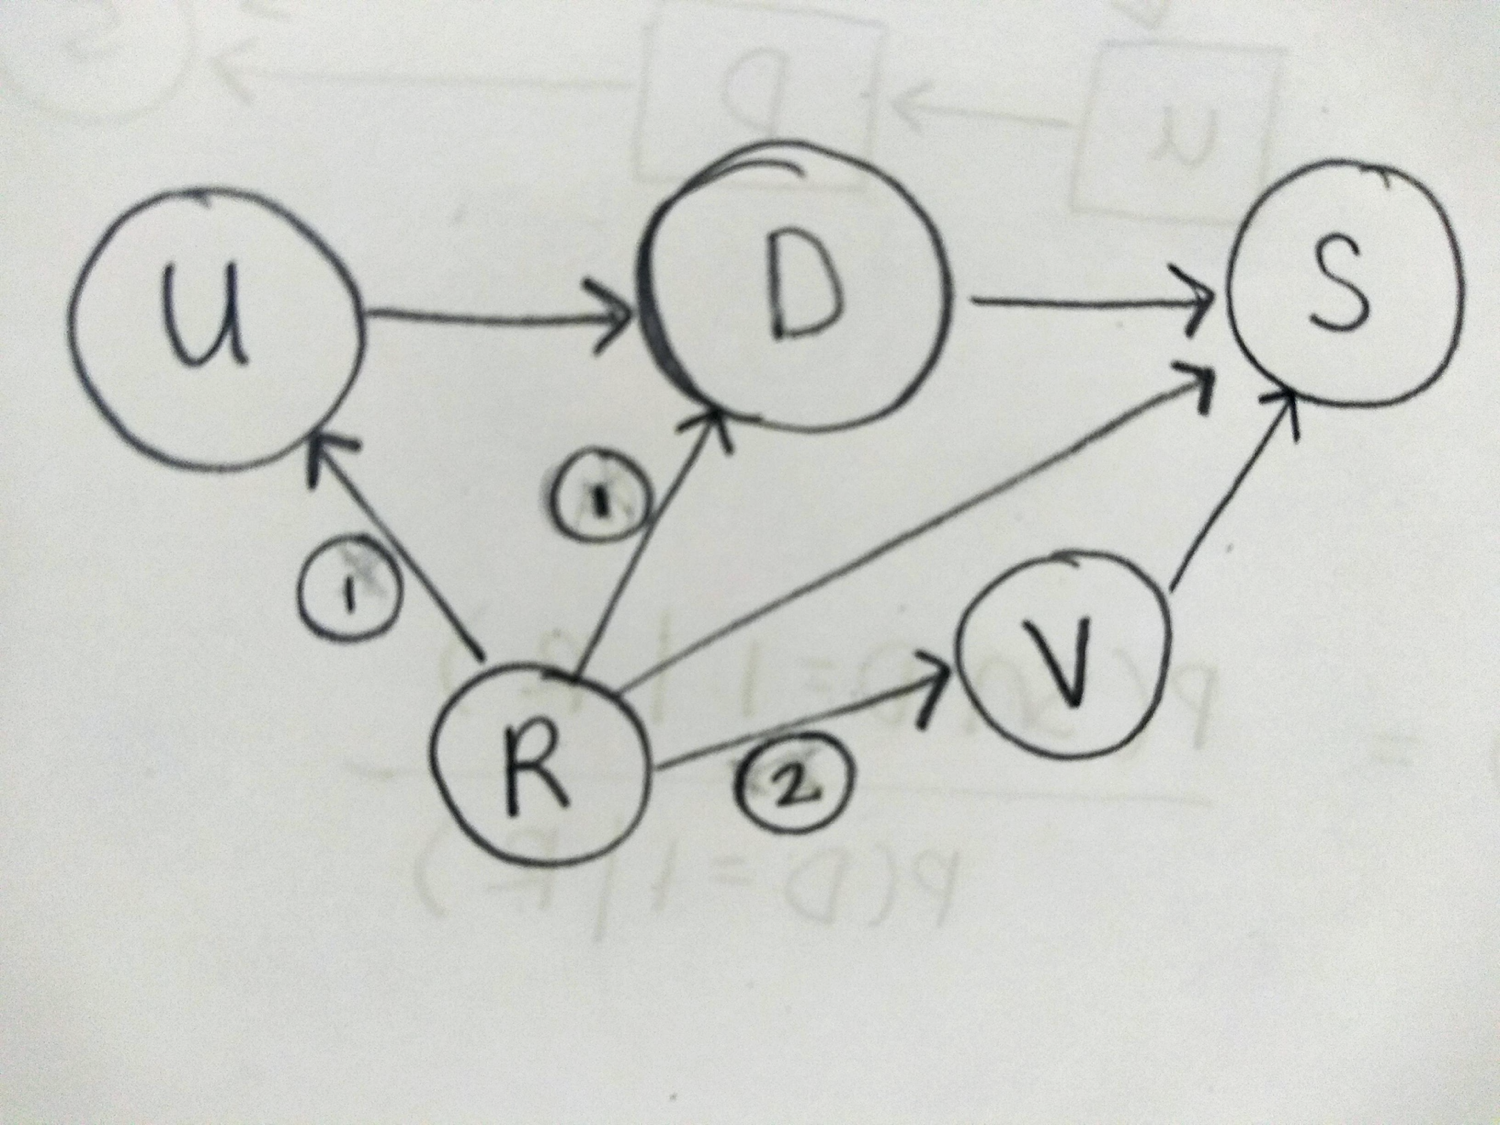
\includegraphics{causal_diagram.png}
\caption{Causal diagram}
\end{figure}

    \question Consider an alternative (``driving while Black'') model in
which the police use race as a criterion for stopping or otherwise
interacting with a given civilian. Compare the causal structure of this
model with your answer to (1). Viewed through the lens of this model,
how would one interpret Fry's failure to reject
\(Pr(S|D = 1, R) = Pr(S|D = 1)\)?

\textbf{Answer} The ``driving while Black'' model explicitly posits what
I call the ``racial profiling'' confounding factor above. If police use
race as a criteran for stopping a civilian, then \(R\) directly
influences \(D\) in the causal diagram, so our ``exclusion restriction''
is violated. Fry fails to reject:

\begin{align*} Pr(S|D = 1, R) &= Pr(S|D = 1) \\ \frac{Pr(S\cap D = 1|R)}{Pr(D=1|R)} &= \frac{Pr(S\cap D = 1)}{Pr(D=1)} \end{align*}

If we suspect that the driving while Black model has relevance here,
then its prediction that \(Pr(D=1|R) > Pr(D=1)\) implies that it is
likely that Fry's estimated probabilities are equal because
\(Pr(S\cap D = 1|R) > Pr(S\cap D = 1)\).

    \question The Justice Department should care about which (Fry's or
the ``driving while Black'') is the better model. How might one go about
testing one against the other?

\textbf{Answer}

The main conflict between these models is that ``driving while Black''
proposes that \(P(D = 1 | R) > P(D = 1)\), whereas Fry's model requires
\(P(D = 1 | R)= P(D = 1)\) for his identification strategy. Therefore,
testing these models against eachother only requires evidence of
\(P(D=1)\) vs.~\(P(D=1|R)\). For example, Horrace and Rohlin (2016)
exploit the relative darkness of night (which deteriorates the ability of
police officers to identify the race of someone they may stop) to
measure racial profiling, and find that the ``odds of a black driver
being stopped (relative to nonblack drivers) increase 15\% in daylight
compared to darkness'' (Horrace and Rohlin, 2016).

References:

William C. Horrace, Shawn M. Rohlin; How Dark Is Dark? Bright Lights,
Big City, Racial Profiling. The Review of Economics and Statistics 2016;
98 (2): 226--232. doi: https://doi.org/10.1162/REST\_a\_00543

\end{questions}

    \hypertarget{weighting-of-linear-iv-estimators}{%
\section{Weighting of Linear IV
Estimators}\label{weighting-of-linear-iv-estimators}}

Consider the Linear IV model
\begin{align*}
y = X\beta + u \qquad\mathbb{E}(Z'u) = 0
\end{align*}

\begin{questions}
    \question Exploiting the moment condition, under what conditions does
the estimator \(b_{IV}\) satisfying \(Z'y = (Z'X)b_{IV}\) consistently
estimate \(\beta\)?

\textbf{Answer} Hansen (2021) outlines the conditions under which \(IV\)
is consistent. The moment conditions already provide the assumption that
\(\mathbb{E}(Z'u) = 0\). Additionally supposing the data is iid, and
that each of \(y, X, Z\) have finite variance, then we only need:

\begin{enumerate}
\def\labelenumi{\arabic{enumi}.}
\tightlist
\item
  \(\mathbb{E}(Z'Z)\) positive definite, and
\item
  \(\mathbb{E}(Z'X)\) full column rank (instrument relevance)
\end{enumerate}

for consistency.

    \question Suppose that \(Z\) has \(l\) columns. Construct a
symmetric, \(l\times l\) full rank matrix \(W\), and a corresponding
estimator \(b_W\) satisfying \(WZ'y = W(Z'X)b_W\). Under what conditions
will this estimator consistently estimate \(\beta\)?

\textbf{Answer} This estimator will consistently estimate \(\beta\) for
any full rank matrix \(W\) such that \(\mathbb{E}(WZ'X)\) is full column
rank, plus the regularity conditions about the data being iid and
\(y, X, Z\) having finite variance.

    \question Describe the GMM criterion function that $b_W$ minimizes.

\textbf{Answer} Let:
\begin{align*}
g_N(\beta) = \sum_{i=1}^N W_iZ_i'y - W_iZ_i'X_i\beta = WZ'y - WZ'X\beta
\end{align*}
then the GMM criterian function is:
\begin{align*}
J(\beta) &= N(WZ'y - WZ'X\beta)'(WZ'y - WZ'X\beta)
\end{align*}
\question Consider Hansen’s description of the two-stage least squares estimator (Section 12.12). What is $W$ for this estimator? Under what conditions is this the optimally weighted GMM estimator?

\textbf{Answer} Minimizing the above, we can see that:
\begin{align*}
J_\beta = -2X'ZW(Z'y - Z'Xb_{gmm}) = 0 \Rightarrow b_{gmm} = (X'ZWZ'X)^{-1}(X'ZWZ'y)
\end{align*}

In two-stage least squares, substituting $\hat{X} = Z(Z'Z)^{-1}Z'X$, we have:
\begin{align*}
b_{2sls} &= (X'Z(Z'Z)^{-1}Z'Z(Z'Z)^{-1}Z'X)^{-1}X'Z(Z'Z)^{-1}Z'y \\
&= (X'Z(Z'Z)^{-1}Z'X)^{-1}X'Z(Z'Z)^{-1}Z'y
\end{align*}

Comparing these two expressions, we can see that $W$ for this estimator is $(Z'Z)^{-1}$. Two stage least squares therefore is the optimally weighted GMM estimator under conditional homoskedasticity, because the scaling does not matter for the weighting matrix, and under conditional homoskedasticity the efficient weighting matrix is $\hat{\Omega}^{-1} = \mathbb{E}(Z'Z)^{-1}$. When distrubances are not homoskedastic, $W = \hat{\Omega}^{-1}$ would take a different form, and these would no longer be equal. 

\question $W = I$ for the $b_{IV}$ estimator described above. Under what conditions is $b_{IV}$ the optimally weighted GMM estimator?

\textbf{Answer} When IV is just identified, the IV and GMM estimators are identical. To see this, note that in the just-identified case, $X'Z$ is a square matrix. Let $\Omega^{-1}$ be the efficient weight matrix for GMM. Then
\begin{align*}
b_{gmm} &= (X'Z\Omega^{-1}Z'X)^{-1}(X'Z\Omega^{-1}Z'y) = (Z'X)^{-1}\Omega(X'Z)^{-1}(X'Z\Omega^{-1}Z'y) \\
 &= (Z'X)^{-1}Z'y = b_{iv}
\end{align*}

Because these estimators are exactly the same and GMM is efficiently weighted, $b_{IV}$ is the efficiently weighted GMM estimator in the just-identified case. This is underscored when examining the variances directly. The variance of the efficiently weighted GMM estimator in the square case reduces to:
\begin{align*}
V_{gmm} = (Z'X)^{-1}\Omega (X'Z)^{-1} = (Z'X)^{-1}Z'ee'Z(X'Z)^{-1} = V_{IV}
\end{align*}


\question For the estimator described in (2), suppose that $W$ is diagonal, with diagonal elements proportional to $(1,1/2,1/4,\ldots,2^{1-l})$. Under what conditions is the estimator $b_W$ the optimally weighted estimator? Can you think of a practical example where the optimal weighting matrix might have this structure?

\textbf{Answer} $b_W$ is the optimally weighted estimator if $W$ is proportional to $(Z'ee'Z)^{-1} = (ZZ'e^2)^{-1}$. 

A practical example where the optimal weighting matrix might have this structure is in the case of serial correlation, parameterized by $\rho$. Suppose that our instruments represent treatment status in time since an event $E$ (think of an event study). If the treatment/event causes the treated to diverge from the untreated over time, then the variance will grow over time, causing the diagonals of $Z'Ze^2$ to grow larger. Subsequently, the diagonals of $(ZZ'e^2)^{-1}$ will decrease by a factor of $\rho$ in each period. 


\end{questions}
    
    
    
\end{document}
